\documentclass[sigconf, review, nonacm, anonymous]{acmart}
% \documentclass[sigconf, nonacm]{acmart}

%% \BibTeX command to typeset BibTeX logo in the docs
\AtBeginDocument{\providecommand\BibTeX{{Bib\TeX}}}

%% Hack to allow for comments about author contribution - not used
% \newcommand{\projectcontrib}[1]{\affiliation{\country{#1}}}

%% If you need any other LaTeX packages, add them here
\usepackage{verbatim}
\usepackage[linesnumbered, boxed, resetcount]{algorithm2e}
\usepackage{microtype}
\let\Bbbk\relax
\usepackage{amsmath,amssymb,amsfonts}
\usepackage{algorithmic}
\usepackage{booktabs}
\usepackage{graphicx}
\usepackage{textcomp}
\usepackage{xcolor}
\usepackage{array}
\usepackage{array}
\usepackage{ragged2e}
\usepackage{subcaption}
\usepackage{float} 
\usepackage{caption}
\captionsetup[figure]{font=small, labelfont=bf, textfont=rm}  % bf=bold title, rm=normal text

\def\BibTeX{{\rm B\kern-.05em{\sc i\kern-.025em b}\kern-.08em
    T\kern-.1667em\lower.7ex\hbox{E}\kern-.125emX}}

    
%% For managing citations, it is recommended to use bibliography files in BibTeX format.
%%
%% You can then either use BibTeX with the ACM-Reference-Format style, or BibLaTeX with the acmnumeric or acmauthoryear sytles, that include support for advanced citation of software artefact from thebiblatex-software package, also separately available on CTAN.

%% print page numbers
\settopmatter{printfolios=true} 

%% end of the preamble, start of the body of the document source.
\begin{document}

%% The "title" command has an optional parameter allowing the author to define a "short title" to be used in page headers.
\title[VISION PRO SURVEILLANCE]{VISION PRO SURVEILLANCE}

%% The "author" command is used to define the authors.
%% You shall sabmit the anonymised version of your paper for review, so no need to include author names here.
% \author{First Awsomeauthor}
% \affiliation{\institution{THWS, MAI}\city{}\country{}}

% \author{Second Greatauthor}
% \affiliation{\institution{THWS, MAI}\city{}\country{}}

% \author{Third Amazingauthor}
% \affiliation{\institution{THWS, MAI}\city{}\country{}}

% %% By default, the full list of authors will be used in the page headers. 
% %% If this is too long use "shortauthors" to define a more concise list with surnames only.
% \renewcommand{\shortauthors}{Awsomeauthor, Greatauthor, Amazingauthor}

%% The abstract is a short summary of the work to be presented in the article.
\begin{abstract}
Recent advances in artificial intelligence (AI) and Internet of Things (IoT) technologies have led to the replacement of traditional locking mechanisms with intelligent, computer vision-based access systems. These systems grant entry exclusively when a registered user is recognized by the camera, thereby automating the unlocking process. However, such systems remain susceptible to spoofing attacks, including the use of 2D photographs or video replays, which compromise security. \\
This paper presents a smart locking system that integrates face recognition with liveness detection to provide secure authentication and prevent spoofing. The system utilizes two ESP-32 camera modules for image acquisition and employs a Raspberry Pi 5 as the primary processing unit. The liveness detection module leverages epipolar geometry to estimate depth between key facial landmarks, preventing spoofing. Upon successful liveness verification, the face recognition module, featuring YuNet for face detection and SFace for recognition, authenticates the user. Once the identity is confirmed, the locking mechanism is disengaged. The lock is actuated through coordinated control of an Arduino, relay, and 12V DC power supply. In addition, an interactive web interface facilitates remote user registration, real-time monitoring, administrative privileges, including user approval and audit logs. The proposed solution offers a cost-effective, robust, and secure smart lock, demonstrating the seamless integration of advanced AI with embedded systems.
\end{abstract}

%% Keywords: pick words that accurately describe the work being presented. Separate the keywords with commas - not used.
\keywords{Computer Vision, Liveliness Detection, Smart Access, Artificial Intelligence, IoT}
%% This command processes the author and affiliation and title information and builds the first part of the formatted document.
\maketitle

%% Add here the link to your code repository
\vspace{-1em}
% \textbf{Code:} \url{https://github.com/PrahasHegde/Face_Recognition_YuNet_SFace}


\section{Introduction}
Smart surveillance systems \cite{mordor2026} play a crucial role in home security by enabling convenient authorized access. However, traditional methods such as PIN codes, RFID cards, and fingerprints are increasingly vulnerable to forgery, cloning, and physical tampering \cite{zainuddin2024}. While existing face recognition algorithms offer a more seamless approach, they remain susceptible to spoofing attacks using high-resolution photos or videos and may struggle in different lighting conditions \cite{bhattacharjee2018}. Furthermore, modern solutions utilize complex machine learning models that improve accuracy but require high computational resources, which limits their use on lightweight platforms like Raspberry Pi and often difficult to scale \cite{yunet2023}. These advanced systems rely on cloud infrastructure for database storage and thus, adds to the financial cost of the entire system.

To overcome these challenges, the proposed system confirms liveness using epipolar geometry and facial landmarks (eyes and nose) to find depth—a lightweight yet effective measure to thwart 2-D spoofing \cite{researchgate2016}. High-speed face detection and recognition are achieved using YuNet and SFace, specifically optimized for resource-constrained environments \cite{yunet2023, deepface2024}. An Arduino to control a solenoid lock, while a web-based dashboard provides live monitoring and remote admin approval \cite{arduinoexpert2025}. Overall, this pipeline achieves a balance between security, accuracy, and performance.

\begin{figure}[t!] 
    \centering
    \Description{Block diagram showing system components: two ESP32 cameras, Raspberry Pi processing, Arduino-actuated solenoid lock, and web dashboard.}
    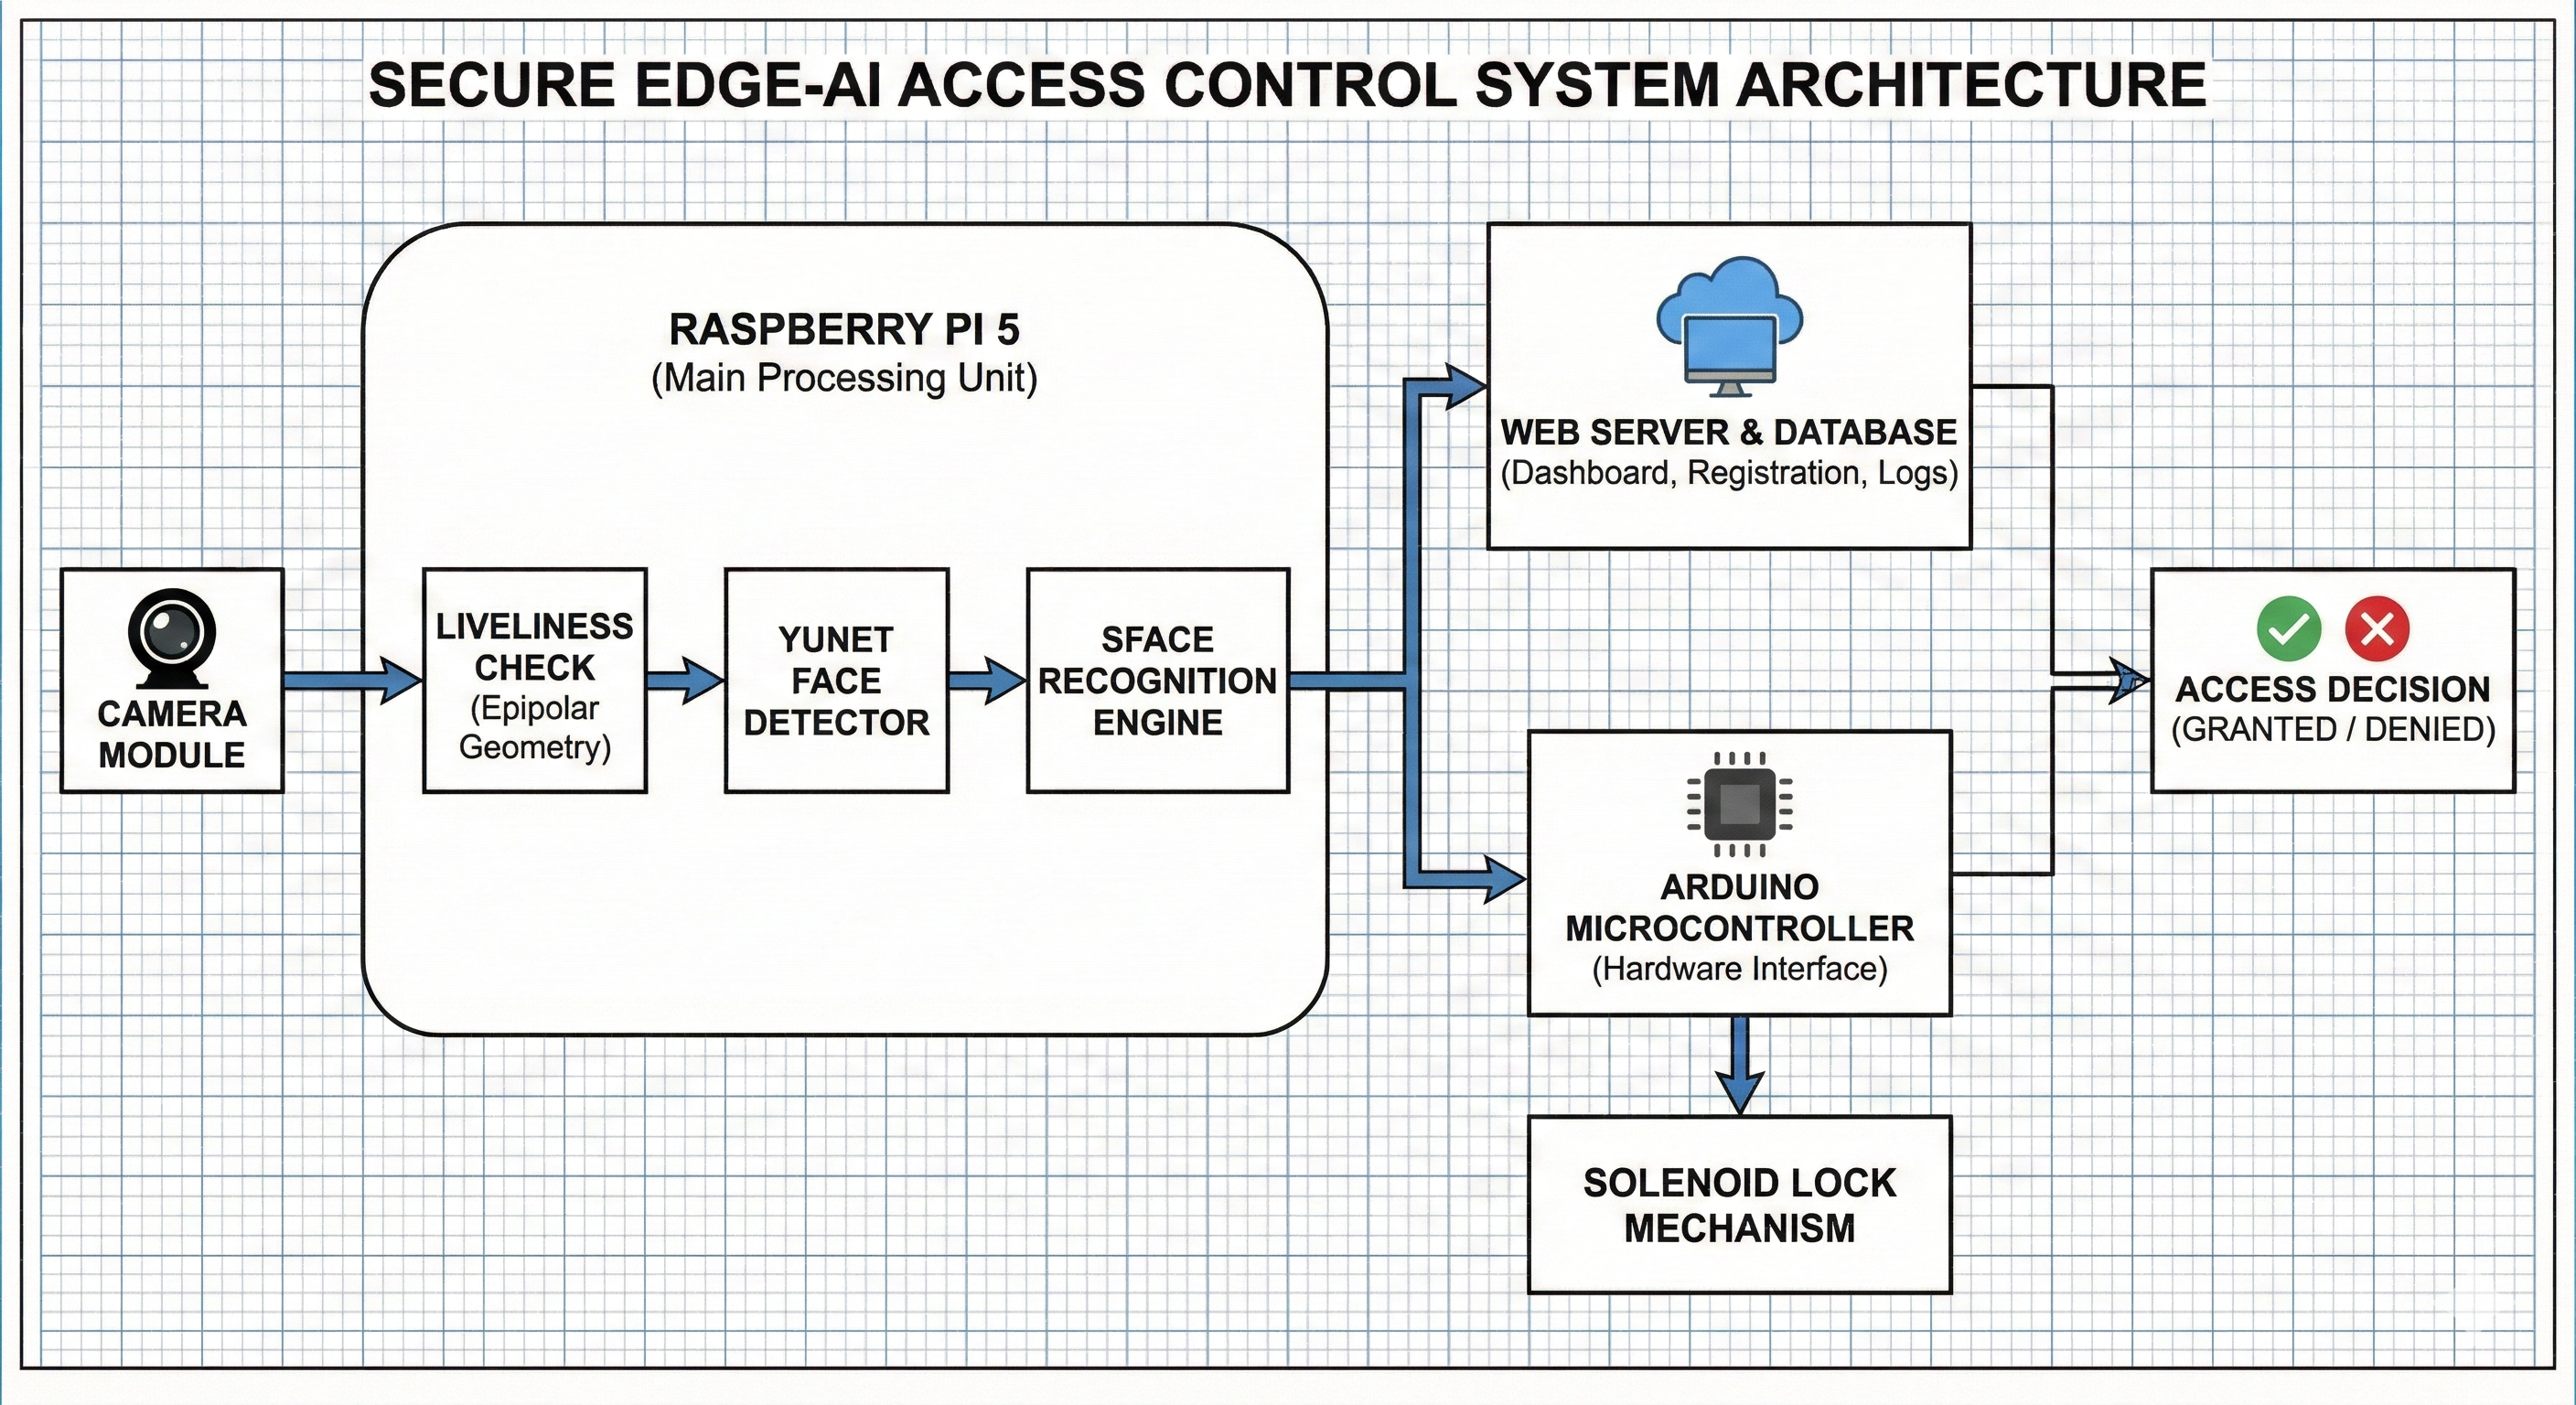
\includegraphics[width=0.45\textwidth]{img/project_bd1.png}
    \caption{\textbf{System Block Diagram:}  An overview of the proposed smart lock, including liveness detection, face recognition, and hardware.}
    \label{fig:system}
\end{figure}

%******************************************************************************

\vspace{-1.5em}
\section{Related Work}
This section reviews existing systems and the computer vision algorithms that underpin our proposed solution.

\subsection{Non-Biometric Smart Locks}
Vongchumyen et al. (2017) proposed a Web-based system and Aswini D. et al. (2021) proposed RFID-OTP systems. While these solve the ``lost key'' problem, they fail to offer true convenience. Wether using a phone app or scanning a tag, the user is required to manually interact with a device, negating the ``hands-free'' benefit of home automation.

\subsection{Monocular Biometric Systems}
To improve convenience, facial recognition was adopted, but single-camera systems face a trade-off between security and speed. Cloud-based solutions (Maheshwari \& Nalini, 2017) offer accuracy but suffer from latency and internet dependency. Alternatively, local offline systems (Elechi et al., 2022) often lack the robustness to distinguish real faces from photos. To counter this, Dasare (2021) introduced ``active liveness'' (hand gestures), which unfortunately adds user friction. A robust system must be both passive (no gestures) and local (offline).

\subsection{Stereo Vision and The Research Gap}
To achieve passive, secure liveness detection, our work leverages Stereo Vision for 3D depth extraction. Our methodology relies on Zhang's (1998) standard for camera calibration to ensure geometric accuracy and Hartley \& Sturm's (1997) triangulation framework to reconstruct facial landmarks. Crucially, we utilize (Hirschmüller 2005) Semi-Global Matching (SGM) algorithm. By applying epipolar geometry constraints, SGM produces dense disparity maps efficiently on embedded hardware. While recent ``Foundation Models'' like (Wen et al.2025) offer high accuracy, they are computationally prohibitive for microcontrollers.


%*********************************************************************************

%*********************************************************************************

\section{Technical Prerequisites}
\label{sec:tech_preq}
This section outlines the mathematical foundations of stereo vision, calibration, and metric learning required for the proposed system.

\subsection{Stereo Calibration \& Epipolar Geometry}
To reconstruct 3D information, we model the camera using the Pinhole Model. First, we estimate the \textbf{Intrinsic Matrix} ($K$) using the flexible calibration technique \cite{Zhang1998}. This accounts for focal length ($f_x, f_y$) and optical center ($c_x, c_y$) from low-cost sensors:

\begin{equation}
    K = \begin{bmatrix} 
    f_x & 0 & c_x \\ 
    0 & f_y & c_y \\ 
    0 & 0 & 1 
    \end{bmatrix}
    \label{eq:intrinsic}
\end{equation}

For stereo consistency, we utilize the \textbf{Epipolar Constraint} and triangulation framework \cite{Hartley1997}. Given a point projected onto the left ($\mathbf{p}_L$) and right ($\mathbf{p}_R$) image planes, their relationship is governed by the Fundamental Matrix ($\mathbf{F}$):

\begin{equation}
    \mathbf{p}_R^T \cdot \mathbf{F} \cdot \mathbf{p}_L = 0
    \label{eq:epipolar}
\end{equation}

\subsection{Disparity \& Depth Estimation}
To compute depth, we first calculate pixel disparity ($d$) using the \textbf{Semi-Global Block Matching (SGBM)} algorithm \cite{hirschmuller2008stereo}. Unlike simple pixel matching, SGBM enforces a global smoothness (WLS) constraint to reduce noise on textureless surfaces like skin. The depth $Z$ is inversely proportional to disparity \cite{Hartley1997}:

\begin{equation}
    Z = \frac{f \cdot B}{d}
    \label{eq:depth}
\end{equation}

Where $Z$ is the distance (depth) of the object from the camera, $f$ is the focal length, $B$ is the baseline distance between cameras, and $d$ is the Disparity ($x_L - x_R$). This relationship allows the system to distinguish between a real face (varying $Z$) and a spoof photograph (constant $Z$).

\subsection{Deep Metric Learning}

Identity verification utilizes a neural network trained with \textbf{Triplet Loss} \cite{Schroff2015} to map facial features into a 128-dimensional embedding space. Verification is performed by calculating the \textbf{Euclidean Distance} between the live embedding ($\mathbf{p}$) and stored embedding ($\mathbf{q}$):

\begin{equation}
    d(\mathbf{p}, \mathbf{q}) = \sqrt{\sum_{i=1}^{128} (p_i - q_i)^2}
    \label{eq:euclidean}
\end{equation}
	
If this distance is below a learned threshold (e.g., $\tau < 0.6$), the identity is confirmed.




%**********************************************************************

\section{Methodology}

\begin{figure*}[t!]
    \centering
    % Left side: 2 small subfigures SIDE-BY-SIDE
    \begin{subfigure}{0.5\textwidth}
        \centering
        \begin{subfigure}{0.39\textwidth}
            \includegraphics[width=\textwidth]{img/mesh2.jpeg}
            \caption{\textbf{3D Reconstruction:} Mesh of facial landmarks with depth.}
            \label{fig:sys1a}
        \end{subfigure}%
        \hspace{0.04\textwidth}%
        \begin{subfigure}{0.45\textwidth}
            \includegraphics[width=\textwidth]{img/disparity.jpeg}
            \caption{\textbf{Disparity:} Disparity map showing depth variations.}
            \label{fig:sys1b}
        \end{subfigure}
    \end{subfigure}%
    \hspace{2em}% 
    \begin{subfigure}{0.45\textwidth}
        \centering
        \includegraphics[width=\textwidth]{img/complx_bd.jpeg}
        \caption{\textbf{Integrated System Architecture: }Sytem components with data flow.}
        \label{fig:sys2}
    \end{subfigure}
    \caption{\textbf{Liveness (3D Reconstruction and Disparity) and Integrated System Architecture.}}
    \label{fig:system}
\end{figure*}




\subsection{System Overview}
The proposed system comprises a sequential processing pipeline designed for real-time secure access control. The workflow begins with stereo vision for depth perception and anti-spoofing, followed by deep learning-based face recognition and a control interface for hardware actuation. The system captures synchronized video streams from two cameras, applies epipolar rectification and depth estimation to verify facial liveness, and subsequently performs identity recognition using learned facial embeddings. After successful authentication, an Arduino-controlled solenoid lock is actuated to grant physical access.

\subsection{System Design and Implementation }
\begin{itemize}
    \item \textbf{Epipolar Geometry:} The stereo vision module follows the calibrated stereo camera model described in Eq.~\ref{eq:intrinsic}. Intrinsic and extrinsic parameters are obtained offline using a standard chessboard calibration procedure. Using these parameters, epipolar rectification is applied to align corresponding scan lines, as in Eq.~\ref{eq:epipolar}. Disparity is then computed along horizontal epipolar lines using the Semi-Global Block Matching (SGBM) algorithm, producing a dense disparity map (Fig.\ref{fig:sys1b}) suitable for real-time processing.

\item \textbf{Depth Estimation:}
The depth (Z) of any pixel is inversely proportional to its disparity (d). The relationship is defined in Eq.\ref{eq:depth}.
The formulation allows reliable estimation of relative facial depth using the calibrated stereo configuration.

\item \textbf{Facial Landmark Localization:}
Facial landmarks are detected using the YuNet model, which identifies both bounding boxes and precise coordinates for key facial features. These landmarks are detected in the rectified image space and mapped to the corresponding coordinates in the disparity map. This mapping enables direct association between facial landmarks and their estimated depth values.

\item \textbf{Liveness Detection:}
A human face is a 3D object where the nose is closer to the camera than eyes. Conversely, a 2D spoof (photo) is planar, meaning the depths of the nose and eyes are approximately equal. Depth values are extracted at the landmark positions corresponding to the left eye, right eye, and nose tip.

\begin{equation}
\Delta Z = \frac{Z_{\text{left\_eye}} + Z_{\text{right\_eye}}}{2} - Z_{\text{nose}}
\end{equation}


where $Z_{\text{left\_eye}}$, $Z_{\text{right\_eye}}$, and $Z_{\text{nose}}$ denote the estimated depths at the corresponding facial landmark. The liveness condition is satisfied if the resulting geometric protrusion exceeds a predefined threshold. To ensure robustness against noise and transient estimation errors, liveness verification is performed over multiple consecutive frames.


\item \textbf{Face Recognition:}
After successful liveness verification, the system employs a deep learning pipeline consisting of two models: YuNet for face detection and SFace for face recognition. To ensure robustness against pose variations, Affine transformation is applied using the facial landmarks provided by YuNet. This transformation aligns the detected face by correcting rotational offsets before it is passed to SFace. SFace converts the aligned facial image into a compact 128-dimensional embedding vector that represents the user’s unique facial characteristics.

Identity matching is performed using cosine similarity:
\begin{equation}
S = \frac{f \cdot g}{\lVert f \rVert \, \lVert g \rVert}
\end{equation}

where $f$ represents the extracted facial feature vector and $g$ denotes a stored enrollment embedding. Access is granted only if the similarity score exceeds a threshold, thereby identifying the user with high confidence.

\item \textbf{Hardware Actuation:}
The system effectively governs transitions between liveness verification, recognition, and access states. Upon successful authentication, a command signal is transmitted via serial communication to an Arduino, which actuates a solenoid lock. A cooldown interval is enforced to prevent repeated triggering.
\end{itemize}


%*********************************************************************************
\vspace{-1em}
\section{Experiments and Evaluation}
\subsection{Dataset}
The initial dataset was collected using a laptop web camera and consists of three subfolders, each corresponding to an individual. Each subfolder contains 200 high-quality images, extracted from a 60-second video in which participants performed various head movements and facial expressions. Images are temporarily stored locally on the Raspberry Pi until they are converted to vector embeddings, ensuring protection from cyber attacks. A Test Dataset consisting of 150 images was used for evaluation.\\ 
Each image is converted into a 128-dimensional vector. The model generates vectors for all training images and averages them to create a 'mean' embedding that represents that person. These embeddings are saved locally in an 'embeddings.pkl' file on the Raspberry Pi 5. The file is used for real-time recognition and model evaluation.

\subsection{Baseline}
In this section, we are conducting a comparative analysis of our model alongside several others. The evaluation framework relies on: \textbf{True Acceptance Rate (TAR)}: system correctly verifies a legitimate user who is enrolled in the database, \textbf{False Acceptance Rate (FAR)}: system incorrectly verifies an unauthorized impostor as a legitimate user \textbf{False Rejection Rate (FRR)}: system incorrectly rejects a legitimate user, failing to recognize their enrolled identity, \textbf{True Rejection Rate (TRR)}: system correctly rejects an unauthorized impostor, denying them access, and \textbf{overall Accuracy}. Our examination includes traditional approaches such as the Haar Cascade Classifier \cite{voilajonas} and the Histogram of Oriented Gradients in conjunction with support vector machine (SVM) \cite{dalaltriggs}. Additionally, we have evaluated deep learning-based models, including the Dlib (OpenCV) \cite{King2009Dlib} and the Insightface (Arcface) \cite{Deng2019ArcFace}.



\subsection{Quantitative Analysis}
The Haar Cascade model demonstrated a very low accuracy (0.08) and a high FRR (0.87). Due to its basic feature-based approach, which is highly susceptible to changes in lighting conditions and non-frontal facial orientations. Similarly, the HOG + SVM was unable to correctly identify most of authorized users (TAR 0.14), likely due to the inflexibility of HOG descriptors when faced with the varied poses and facial expressions present in the test set.

Among the deep learning approaches, Dlib (OpenCV) achieved improved recognition performance (TAR 0.83), but it was accompanied by a significant security concern: (FAR 0.55). This indicates lack of discriminative ability to differentiate between users and impostors. Although InsightFace demonstrated high accuracy (0.94), it was not selected due to hardware constraints. Its computationally intensive architecture exceeded the capabilities of the Raspberry Pi 5 and rendered it unsuitable for edge deployment.\\

\vspace{-1em}
% -----------------------------
% Table 
% -----------------------------

\begin{table}[htbp]
\centering
\caption{Model Evaluation}
\begin{tabular}{lccccc}
\toprule
\textbf{Models} & \textbf{TAR} & \textbf{FAR} & \textbf{FRR} & \textbf{TRR} & \textbf{Accuracy} \\
\midrule
Haar Cascade & 0.13 & 0.70 & 0.87 & 0.3 & 0.08 \\
HOG + SVM & 0.14 & 0.13 & 0.86 & 0.87 & 0.52 \\
Dlib (OpenCV) & 0.83 & 0.55 & 0.0 & 0.45 & 0.60 \\
Insightface\textsuperscript{*} & 0.90 & 0.0 & 0.10 & 1.0 & 0.94 \\
YuNet + SFace (Ours) & 1.0 & 0.0 & 0.0 & 1.0 & 1.0 \\
\bottomrule
\end{tabular}
\label{tab:metric evaluation}
\end{table}

\vspace{-0.5em}
\begin{flushleft}
\footnotesize * indicates that the training/testing was conducted on a PC instead of the Raspberry Pi 5, due to the computational intensity.
\end{flushleft}
 
Ultimately, YuNet + SFace provided the optimal solution. It achieved perfect metrics (1.0 Accuracy, 0.0 FAR), demonstrating the ideal balance of computational efficiency and high-precision security required for the final system.





\begin{figure}[t!]
    \centering
    \Description{Confusion matrix or comparative chart showing model performance across tested configurations.}
    \includegraphics[width=0.35\textwidth]{img/model_cf.png}
    \caption{\textbf{Confusion Matrix for YuNet + SFace:} Demonstrating perfect accuracy and low error.}
    \label{fig:cf}
\end{figure}


% -----------------------------
% Table 
% -----------------------------
\begin{table}[htbp]
\centering
\caption{Ablation Study}
\footnotesize
\begin{tabular}{lccc>{\RaggedRight}p{2.5cm}}
\toprule
\textbf{Configuration} & \textbf{Accuracy} & \textbf{FAR} & \textbf{Latency} & \textbf{Comments} \\
\midrule
YuNet + LBPH & 0.85 & 0.80 & 18 ms & Good cropping cannot fix LBPH's texture limitations. \\
Haar Cascade + SFace & 0.68 & 0.05 & 14 ms & Good recognizer limited by Haar's inability to find faces. \\
Retinaface + Arcface\textsuperscript{*} & 1.0 & 0.0 & 180 ms & Accurate but impractical for real-time use. \\
YuNet + SFace (ours) & 1.0 & 0.0 & 15 ms & \textbf{Optimal}, perfect balance of speed, size, and security. \\
\bottomrule
\end{tabular}
\label{tab:ablation}
\end{table}



To further validate our proposed system, we conducted an ablation study to isolate the impact of the detector (YuNet) and the recognizer (SFace) independently. We tested four configurations: YuNet + LBPH, Haar Cascade + SFace, Retinaface + Arcface, and the proposed YuNet + SFace.
We first assessed the texture-based recognizer by evaluating the YuNet + LBPH. Despite the integration of a robust detector, system accuracy decreased to 0.45, accompanied by a high FAR (0.40). These results indicates, Local Binary Pattern Histograms (LBPH) lack the necessary feature extraction depth for secure identification.

In contrast, we explored a less robust detector by pairing Haar Cascade with SFace. Although this setup achieved low latency (14 ms), the accuracy was constrained to 0.68. The system performance was hindered by the Haar Cascade detector's frequent failure to detect faces, resulting in a significant bottleneck. These findings confirm that traditional detectors are inadequate for providing reliably consistent input to the recognition pipeline.

The Retinaface + Arcface configuration matched our model's perfect accuracy (1.0) and FAR (0.0), it suffered from a massive latency penalty, taking 180 ms per frame. This is over 10 times slower than our proposed solution, making it impractical for real-time edge applications where rapid response is critical.\\

The YuNet + SFace configuration emerged as the optimal architecture. It achieved perfect accuracy (1.0) and security (0.0 FAR) and also maintained an ultra-low latency of 15 ms. This confirms that YuNet + SFace successfully bridges the gap between high-performance security and real-time efficiency, validating its selection as the core engine for our embedded system.






\subsection{Qualitative Analysis}


% -----------------------------
% Table I
% -----------------------------
\begin{table}[htbp]
\centering
\caption{Expected Depth Differences}
\begin{tabular}{l>{\centering\arraybackslash}p{4cm}}
\toprule
\textbf{Classification} & 
\textbf{$\Delta z$ (m)} \\
\midrule
Average Adult Face  & 0.020--0.030 \\
Average Child Face  & 0.015--0.020 \\
Photo / Flat Surface & $\approx 0.000$ \\
\bottomrule
\end{tabular}
\label{tab:depth_differences}
\end{table}


\noindent \textbf{Table~\ref{tab:depth_differences}} shows expected depth differences for real human faces and planar surfaces. These theoretical values form the basis for liveness detection.


% -----------------------------
% Table II
% -----------------------------
\begin{table}[htbp]
\caption{Liveness Decision Parameters}
\centering
\begin{tabular}{lc}
\toprule
\textbf{Parameter} & \textbf{Value} \\
\midrule
Liveness Minimum ($\Delta Z_{\min}$) & 0.015 m \\
Liveness Maximum ($\Delta Z_{\max}$) & 0.080 m \\
Consensus Frames ($N_c$) & 3 \\
\bottomrule
\end{tabular}
\label{tab:liveness_params}
\end{table}

\noindent \textbf{Table~\ref{tab:liveness_params}} lists the  Liveness Decision parameters. The depth thresholds define valid liveness ranges, and the consensus frame count ensures stability across multiple frames.

% -----------------------------
% Table III
% -----------------------------
\begin{table}[htbp]
\caption{Depth Measurements and Liveness Results}
\centering
\begin{tabular}{lcccc}
\toprule
\textbf{Test Scenario} & \textbf{$Z_{eyes}$ (m)} & \textbf{$Z_{nose}$ (m)} & \textbf{$\Delta Z$ (m)} & \textbf{Result} \\
\midrule
Real Human Subject & 0.430 & 0.393 & \textbf{0.037} & \textbf{PASS} \\
Printed Photo & 0.338 & 0.335 & 0.003 & FAIL \\
Mobile Phone Screen & 0.477 & 0.356 & 0.121 & FAIL \\
\bottomrule
\end{tabular}
\label{tab:results}
\end{table}

\noindent \textbf{Table~\ref{tab:results}} compares measured depth differences for real faces and spoof attacks. Human faces fall within the liveness range and pass the test, while printed photos and phone screens fail due to inconsistent depth variation. Mobile phone screens show higher depth differences than expected for a planar surface because reflections, and display curvature introduce erroneous stereo disparities, which the system interprets as depth variation, resulting in artificially inflated Z values. Despite this, the values remain outside the valid liveness range, so the spoof is correctly rejected.

%*******************************************************************

\section{Conclusion}
This research presents an efficient real-time face recognition system for edge computing on the Raspberry Pi 5, featuring epipolar geometry-based liveness detection and a web management dashboard. The YuNet + SFace pipeline outperformed other models, demonstrating that high-precision biometric authentication is feasible on affordable embedded hardware.

%**********************************************************************
\section{Acknowledgment}
We would like to express our sincere gratitude to the  Technical University of Applied Sciences Würzburg-Schweinfurt (THWS) for providing the academic environment, infrastructure, and resources necessary to carry out this project.
We also extend our heartfelt thanks to Prof. Dr. Andreas Lehrmann for his valuable guidance, continuous support, and insightful feedback throughout the development of this work. His expertise and encouragement played a crucial role for the successful implementation.

\bibliographystyle{ACM-Reference-Format}
\bibliography{references}


\end{document}